\documentclass[10pt,a4paper]{article}
\usepackage[utf8]{inputenc}\usepackage[T1]{fontenc}\usepackage[german]{babel}
\usepackage{graphicx,float,booktabs,amsmath,siunitx,xcolor,tabularx}
\usepackage[margin=2.2cm]{geometry}\usepackage[hidelinks]{hyperref}
\sisetup{output-decimal-marker={,}}
\hypersetup{pdfauthor={Thomas Schmiegelt},pdftitle={Ein Ersatzmodell für Stellarator-Spulengehäuse}}
\newcommand{\bild}[3]{\begin{figure}[H]\centering\includegraphics[width=#2\linewidth]{bilder/#1}\caption{#3}\end{figure}}
\newcommand{\zwei}[3]{\begin{figure}[H]\centering\includegraphics[width=0.49\linewidth]{bilder/#1}\hfill
  \includegraphics[width=0.49\linewidth]{bilder/#2}\caption{#3}\end{figure}}
\newcommand{\kasten}[2]{\par\smallskip\noindent\fcolorbox{gray}{gray!8}{\parbox{0.96\linewidth}{\textbf{#1} #2}}\par\smallskip}
\title{\textbf{Ein Ersatzmodell für Stellarator-Spulengehäuse}\\[2pt]\large Von 157 FEM-Rechnungen zur
  Vorhersage in Millisekunden -- mit einem lokalen KI-Agenten als Aufsicht}
\author{Thomas Schmiegelt \textbar{} Hobbyprojekt \texttt{stellarator-design}}
\date{25.10.2026}
\begin{document}\maketitle

\kasten{Hobbyprojekt, aus Neugier entstanden.}{Keine Verbindung zu einem Forschungsinstitut oder Unternehmen,
nicht begutachtet. Alle Zahlen sind Abschätzungen mit vereinfachten Modellen und können Fehler enthalten. Das
W7-X-Modell ist \emph{angelehnt an} Wendelstein~7-X: Die Spulenbahnen stammen aus öffentlichen Daten
\cite{simsopt}; Gehäuse, Verbinder, Verguss, Lagerung und Wandstärken sind eigene, vereinfachte Annahmen und
entsprechen nicht der realen Anlage. Die 1-GW-Anlage ist ein eigener Entwurf. Programmcode, Rechnungen und
Textentwurf entstanden mit Unterstützung von KI-Agenten; alle Abbildungen sind eigene Rechnungen.}

\begin{abstract}
Dieser Bericht setzt den Projektbericht fort. Dort entstand eine Rechenkette von der Spulenbahn bis zur
Vergleichsspannung im Gehäuse; eine Rechnung dauert Minuten. Für Variantenstudien ist das zu langsam. Deshalb
wurde ein \emph{Ersatzmodell} (Surrogat) gebaut: Ein Hex-Netz fester Topologie mit Wickelpaket, Verguss,
Stahlgehäuse und Verbindern wird über einen Versuchsplan je Anlage 78- bzw.\ 79-mal mit ElmerFEM gerechnet, danach lernt
ein Gauß-Prozess die Kennzahlen und ein reduziertes Modell die Spannungs- und Verformungsfelder. Zwei Anlagen
wurden behandelt: eine W7-X-ähnliche mit dem Feld auf der Achse $B_0$ als Lastgröße und ein eigener
1-GW-Entwurf mit der elektrischen Netzleistung als Lastgröße. Die Kennzahlen 99-\%-Spannung, Mittelwert,
Masse und Verformung werden mit $R^2>0{,}98$ und wenigen Prozent Fehler vorhergesagt; Spitzenwerte einzelner
Elemente nur auf etwa \SI{15}{\%}. Den mehrstündigen Rechenlauf überwachte ein lokal betriebener KI-Agent,
der nur eine Steuerdatei ändern durfte. Ergebnis in der Sache: Bei der W7-X-ähnlichen Anlage entscheiden die
Seitenwände, bei der 1-GW-Anlage reichen Einzelgehäuse mit Verbindern grundsätzlich nicht.
\end{abstract}

\tableofcontents

%======================================================================
\section{Warum ein Ersatzmodell?}
Ein Konstrukteur will Fragen stellen wie: \emph{Was bringt \SI{1}{cm} mehr Seitenwand? Wie viel Stahl kostet
eine Halbierung der Verformung? Wie ändert sich das Bild, wenn die Anlage auf \SI{1,4}{GW} wächst?} Jede
Antwort braucht viele Rechnungen. Eine FEM-Rechnung des ganzen Spulensystems dauert hier eine bis zwei Minuten
und belegt viel Arbeitsspeicher; das Ersatzmodell antwortet in Millisekunden und gibt zusätzlich an, wie sicher
es sich ist.

Das Vorgehen folgt dem üblichen Muster: \textbf{Geometrie bauen} $\to$ \textbf{Parameter festlegen} $\to$
\textbf{Versuchsplan rechnen} $\to$ \textbf{trainieren} $\to$ \textbf{prüfen}. Neu gegenüber dem Projektbericht
sind Verguss und Verbinder im Modell sowie die Steuerung des Laufs durch einen lokalen KI-Agenten.

%======================================================================
\section{Rechenmodell}
\subsection{Netz fester Topologie}
Ein Ersatzmodell, das ganze Felder lernt, braucht für jede Variante dasselbe Netz: gleiche Knotenzahl, gleiche
Reihenfolge, nur die Koordinaten ändern sich. Deshalb wird das Netz nicht mit einem Vernetzer erzeugt, sondern
direkt als strukturiertes Hexaedernetz im Elmer-Format geschrieben. Entlang jeder Spulenbahn liegen
Querschnitte (64 Stationen bei W7-X, 96 bei der 1-GW-Anlage); jeder Querschnitt ist ein Tensorgitter
\emph{Wand | Verguss | Wickelpaket | Verguss | Wand} mit 10 Zellen je Richtung. Wandstärken und Vergussdicke
verschieben nur Knoten.

\kasten{Verbinder.}{Benachbarte Spulen werden durch Hex-Brücken zwischen einander zugewandten Seitenflächen
verbunden. Damit die Topologie fest bleibt, wird der Verbinderplan einmal aus 24 Testgeometrien über den ganzen
Parameterbereich bestimmt und dann für alle Proben verwendet. Zuerst entstanden Verbinder auch zwischen sich
kreuzenden Spulen -- mit umgestülpten Elementen. Diese Fehler fielen anfangs nicht auf, weil die Prüfung der
Jacobi-Determinante das Vorzeichen doppelt aufhob. Nach der Korrektur wurden 15 schon gerechnete Proben
verworfen.}

\subsection{Last und Lösung}
Die Lorentzkraft $\mathbf f = \mathbf J\times\mathbf B$ wird mit Biot-Savart über $4\times4$ Teilleiter je
Spule berechnet und als Knotenkraftdichte über eine kleine Fortran-Funktion an Elmer \cite{elmer} übergeben. Die
Funktion prüft beim Einlesen, ob die Knotenreihenfolge zum Netz passt. Kontrolle: Nettokraft auf eine Spule
\SI{2,36}{MN} gegenüber \SI{2,39}{MN} aus der unabhängigen Feldrechnung ($-1{,}3\,\%$).

Gelöst wird nur die lineare Elastizität. Das iterative Verfahren (CG mit ILU0) konvergierte auf diesem Netz
nicht; der direkte Löser MUMPS \cite{mumps} läuft zuverlässig. Eine Probe dauert etwa \SI{90}{s} (W7-X,
\num{545000} Knoten) bzw. \SI{40}{s} (1 GW, \num{190000} Knoten). Ausgewertet werden die von-Mises-Spannung je
Element und Werkstoff sowie die Verformung.

\subsection{Zwei Anlagen, zwei Lastgrößen}
\begin{table}[H]\centering\small
\begin{tabularx}{\linewidth}{@{}lXX@{}}\toprule
 & W7-X-ähnlich & 1-GW-Entwurf (qa\_nfp2\_A45, HTS) \\\midrule
Spulen & 70 (50 nichtplanar, 20 planar) & 16 \\
Lastgröße & $B_0$ = 1,5 \ldots\ 3,0\,T & Netzleistung 600 \ldots\ 1400\,MW \\
Lastabbildung & Kraft $\propto B_0^2$ (eine Rechnung bei 2,5\,T) & Stufe-0-Bilanz: $P$ $\to$ $R_0$, $B_0$,
  Wickelpaket, Strom \\
Wand innen / seitlich & 2 \ldots\ 8\,cm & 10 \ldots\ 60 / 8 \ldots\ 40\,cm \\
Wand außen ($t_\text{min}$ + Zusatz) & 2 \ldots\ 10 + 0 \ldots\ 15\,cm & 15 \ldots\ 80 + 0 \ldots\ 60\,cm \\
Verguss & 2 \ldots\ 20\,mm, $E$ = 3 \ldots\ 20\,GPa & 5 \ldots\ 50\,mm, $E$ = 3 \ldots\ 20\,GPa \\
Verbinder & $E$ = 1 \ldots\ 200\,GPa & $E$ = 1 \ldots\ 200\,GPa \\
Lagerflecken-Radius & 0,25 \ldots\ 1,0\,m & 1 \ldots\ 4\,m \\\bottomrule
\end{tabularx}\caption{Parameterbereiche des Versuchsplans. Der E-Modul von Verguss und Verbinder wird
logarithmisch abgetastet.}\end{table}

Bei der 1-GW-Anlage legt eine einfache Leistungsbilanz (Stufe 0) zu jeder Netzleistung die Anlagengröße fest.
Mit steigender Leistung wächst der große Radius von \SI{8,2}{m} auf etwa \SI{12}{m}, während das Feld auf der
Achse von \SI{8,5}{T} auf unter \SI{6}{T} sinkt; der Spulenstrom bleibt fast gleich (\SI{23}{MA}). Das erklärt
weiter unten, warum die Spannung mit der Leistung \emph{fällt}.

\zwei{probe0_w7x.png}{probe0_1gw.png}{Mittelpunkt des Versuchsplans, von-Mises-Spannung im Stahl (FEM).
Links W7-X-ähnlich bei \SI{2,5}{T}, rechts 1-GW-Anlage bei \SI{1000}{MW}.}

%======================================================================
\section{Versuchsplan und Training}
Je Anlage wurde ein Latin-Hypercube-Plan \cite{mckay1979} mit 150 Punkten erstellt; Probe 0 ist die
Bereichsmitte. In der verfügbaren Zeit wurden 78 (W7-X) bzw.\ 79 (1 GW) Proben gerechnet. Bei der 1-GW-Anlage fiel eine Probe wegen
umgestülpter Verbinder-Elemente aus; eine weitere, durch einen Bedienfehler abgebrochene, wurde nachgerechnet. Trainiert wurde mit scikit-learn \cite{sklearn}:
\begin{itemize}
\item \textbf{Kennzahlen:} je ein Gauß-Prozess \cite{rasmussen2006} (Matérn-Kern, $\nu=2{,}5$) auf dem Logarithmus
  der Kennzahl; die Streuung des Prozesses liefert einen Unsicherheitsfaktor.
\item \textbf{Felder:} Hauptkomponentenzerlegung (POD) der Spannungs- und Verschiebungsfelder aller Proben
  (20 bzw. 12--15 Moden), je Mode ein Gauß-Prozess. So entsteht in Millisekunden ein ganzes 3D-Feld.
\end{itemize}
Geprüft wurde mit fünffacher Kreuzvalidierung: Jede Probe wird von einem Modell vorhergesagt, das sie nicht
gesehen hat.

\begin{table}[H]\centering\small
\begin{tabular}{@{}lrrrr@{}}\toprule
 & \multicolumn{2}{c}{W7-X-ähnlich} & \multicolumn{2}{c}{1 GW} \\
Kennzahl & $R^2$ & Medianfehler & $R^2$ & Medianfehler \\\midrule
Stahl, 99-\%-Wert von Mises & 0,992 & 1,3\,\% & 0,981 & 2,3\,\% \\
Stahl, Mittelwert & 0,995 & 1,1\,\% & 0,996 & 1,2\,\% \\
Stahlmasse & 0,996 & 0,6\,\% & 0,998 & 0,9\,\% \\
größte Verformung & 0,984 & 2,8\,\% & 0,981 & 3,9\,\% \\
Wickelpaket, 99-\%-Wert & 0,988 & 2,1\,\% & 0,904 & 6,0\,\% \\
Verguss, 99-\%-Wert & 0,982 & 2,4\,\% & 0,875 & 4,5\,\% \\
Verbinder, Maximum & 0,995 & 3,0\,\% & 0,974 & 8,5\,\% \\
Stahl, Maximum (ein Element) & 0,41 & 11,7\,\% & 0,67 & 14,8\,\% \\
Verguss, Maximum (ein Element) & 0,57 & 15,2\,\% & 0,61 & 12,0\,\% \\\bottomrule
\end{tabular}\caption{Kreuzvalidierung, 78 bzw.\ 79 Proben.}\end{table}

\kasten{Lesart für die Praxis.}{Spitzenwerte einzelner Elemente hängen an Kanten und Verbinderanschlüssen und
sind auch in der FEM netzabhängig; sie taugen nicht als Zielgröße für ein Ersatzmodell. Der 99-\%-Wert ist
robust und wird sehr gut getroffen. Für eine Festigkeitsbewertung wären Kerbstellen ohnehin gesondert und feiner
zu rechnen.}

\bild{validierung_w7x.png}{1.0}{Kreuzvalidierung W7-X-ähnlich: Surrogat über FEM. Die beiden Maxima (links oben,
Mitte unten) streuen, alle anderen Kennzahlen liegen auf der Diagonalen.}

\subsection{Gegenprobe außerhalb des Versuchsplans}
Zusätzlich wurde für die 1-GW-Anlage ein neuer Punkt nahe am Rand des Bereichs vorhergesagt und anschließend
mit FEM gerechnet (\SI{1000}{MW}, Wand innen \SI{50}{cm}, seitlich \SI{30}{cm}, Lagerradius \SI{3,5}{m}):

\begin{table}[H]\centering\small
\begin{tabular}{@{}lrrr@{}}\toprule
Kennzahl & Surrogat & FEM & Abweichung \\\midrule
Stahl, 99-\%-Wert & \SI{2490}{MPa} & \SI{2514}{MPa} & $-0{,}9\,\%$ \\
Stahl, Mittelwert & \SI{560}{MPa} & \SI{566}{MPa} & $-1{,}1\,\%$ \\
Stahlmasse & \SI{11078}{t} & \SI{11013}{t} & $+0{,}6\,\%$ \\
größte Verformung & \SI{737}{mm} & \SI{761}{mm} & $-3{,}1\,\%$ \\
Wickelpaket, 99-\%-Wert & \SI{887}{MPa} & \SI{1039}{MPa} & $-14{,}6\,\%$ \\
Verbinder, Maximum & \SI{830}{MPa} & \SI{1003}{MPa} & $-17{,}3\,\%$ \\
Stahl, Maximum & \SI{6676}{MPa} & \SI{7924}{MPa} & $-15{,}8\,\%$ \\\bottomrule
\end{tabular}\caption{Gegenprobe 1-GW-Anlage. Das Surrogat unterschätzt hier die lokalen Werte.}\end{table}

\bild{vorhersage_1gw.png}{0.8}{Vom Surrogat vorhergesagtes Spannungsfeld der Gegenprobe (1 GW). Die Verbinder
(Querstege) sind kaum belastet, die Spitzen liegen an den Innenseiten der Spulen.}

%======================================================================
\section{Was das Ersatzmodell zeigt}
\bild{auswertung.png}{1.0}{Oben W7-X-ähnlich, unten 1-GW-Anlage. Links Spannungen über der Last, Mitte
Verformung, rechts Empfindlichkeit des 99-\%-Werts im Stahl, wenn ein Parameter allein von der unteren zur oberen
Grenze geht. Alle übrigen Parameter in Bereichsmitte.}

\paragraph{W7-X-ähnlich.} Die Spannungen wachsen erwartungsgemäß mit $B_0^2$: Bei \SI{2,5}{T} liegt der
99-\%-Wert im Stahl bei etwa \SI{470}{MPa}, bei \SI{3}{T} bei etwa \SI{680}{MPa}; die Verformung erreicht
\SIrange{27}{39}{mm}. Größter Hebel ist die \textbf{Seitenwand} ($+50\,\%$ Spannung bei \SI{2}{cm}, $-20\,\%$
bei \SI{8}{cm}), dann die Innenwand. Ein dickerer Verguss \emph{erhöht} den Stahlwert leicht -- er leitet mehr
Kraft konzentriert in die Wand. Lagerradius und E-Moduln von Verguss und Verbinder spielen kaum eine Rolle.
Diese Zahlen gelten für eine stark vereinfachte Lagerung (ein eingespannter Flecken je Spule); sie liegen deutlich
über dem früheren Tetraedermodell (\SI{110}{MPa}). Der Widerspruch ist offen (Befund B-027) und betrifft
vermutlich Lagerung und Lastaufbringung.

\paragraph{1 GW.} Hier liegt der 99-\%-Wert im ganzen Bereich bei \SIrange{3,1}{3,7}{GPa}, weit über jedem
Baustahl -- trotz Wänden bis \SI{60}{cm} und knapp \num{9000}~t Stahl. Die Spannung fällt mit steigender Leistung,
weil die Stufe-0-Auslegung größere Anlagen mit niedrigerem Feld wählt. Die Verformung liegt bei fast einem Meter.
Anders als bei W7-X wirkt hier auch die Steifigkeit der Verbinder ($\pm 20\,\%$). \textbf{Folgerung:} Einzelne
Gehäuse, punktuell verbunden, tragen \SI{1,2}{GN} je Spule nicht. Es braucht eine durchgehende Stützstruktur,
wie sie in großen Entwürfen als geschlossener Stützring oder gemeinsames Gehäuse vorgesehen ist.

%======================================================================
\section{Ausblick: Gitterstrukturen}
Aus der Folgerung für die 1-GW-Anlage entstand die Idee, den Raum zwischen den Gehäusen mit einer
Gitterstruktur zu füllen. Gitter aus dem Programm PicoGK \cite{picogk} lassen sich nicht direkt in das große Netz
übernehmen. Deshalb ein Zweistufen-Vorgehen: zuerst die effektive Steifigkeit einer Einheitszelle rechnen, dann
das Gitter im großen Modell als verschmiertes Material mit der Dichte als neuem Parameter einsetzen.

Stufe~1 ist begonnen: PicoGK baut Einheitszellen (raumzentriertes Stabgitter BCC und Gyroid-Schale), die als
Voxel-Hexnetz mit Elmer unter einachsigem Druck gerechnet werden. Die Kennlinien folgen dem bekannten Gesetz
$E^*/E_s = C\,\rho^n$ \cite{gibson1997}: für BCC $n\approx 2{,}55$ (biegedominiert), für das Gyroid $n\approx1{,}46$.
Bei gleicher Dichte ist das Gyroid drei- bis fünfmal steifer. Zugleich hat es die größere spezifische Oberfläche
(\SIrange{530}{600}{m^2/m^3} bei \SI{10}{mm} Zelle, gegenüber \SIrange{180}{330}{m^2/m^3} bei BCC) -- interessant
für die zweite Aufgabe: Die Wand des Plasmagefäßes muss Wärme abführen und Wasser zum Sieden bringen.

\zwei{zellen_galerie.png}{gitter_kennlinie.png}{Links: Einheitszellen aus PicoGK. Rechts: effektiver E-Modul
über der relativen Dichte ($E_s$ = \SI{200}{GPa}). Nur Druck in einer Richtung; der volle Steifigkeitstensor
(Schub, Querrichtungen) steht noch aus.}

Als erste Anschauung dieser zweiten Aufgabe wurde die Gefäßwand der 1-GW-Anlage als \SI{0,9}{m} dicke Doppelhaut
mit Gyroid-Kern (Zelle \SI{0,6}{m}, rund 25\,\% Stahl) in PicoGK gebaut, je \ang{10}-Segment ein Lauf, und mit
den Spulengehäusen aus dem Surrogat in Blender \cite{blender} gerendert (Abb.~\ref{fig:gyroidgefaess}). Das ist eine
Darstellung, keine Auslegung: Strömung, Wärmeübergang und Festigkeit des Kerns sind nicht gerechnet.

\begin{figure}[H]\centering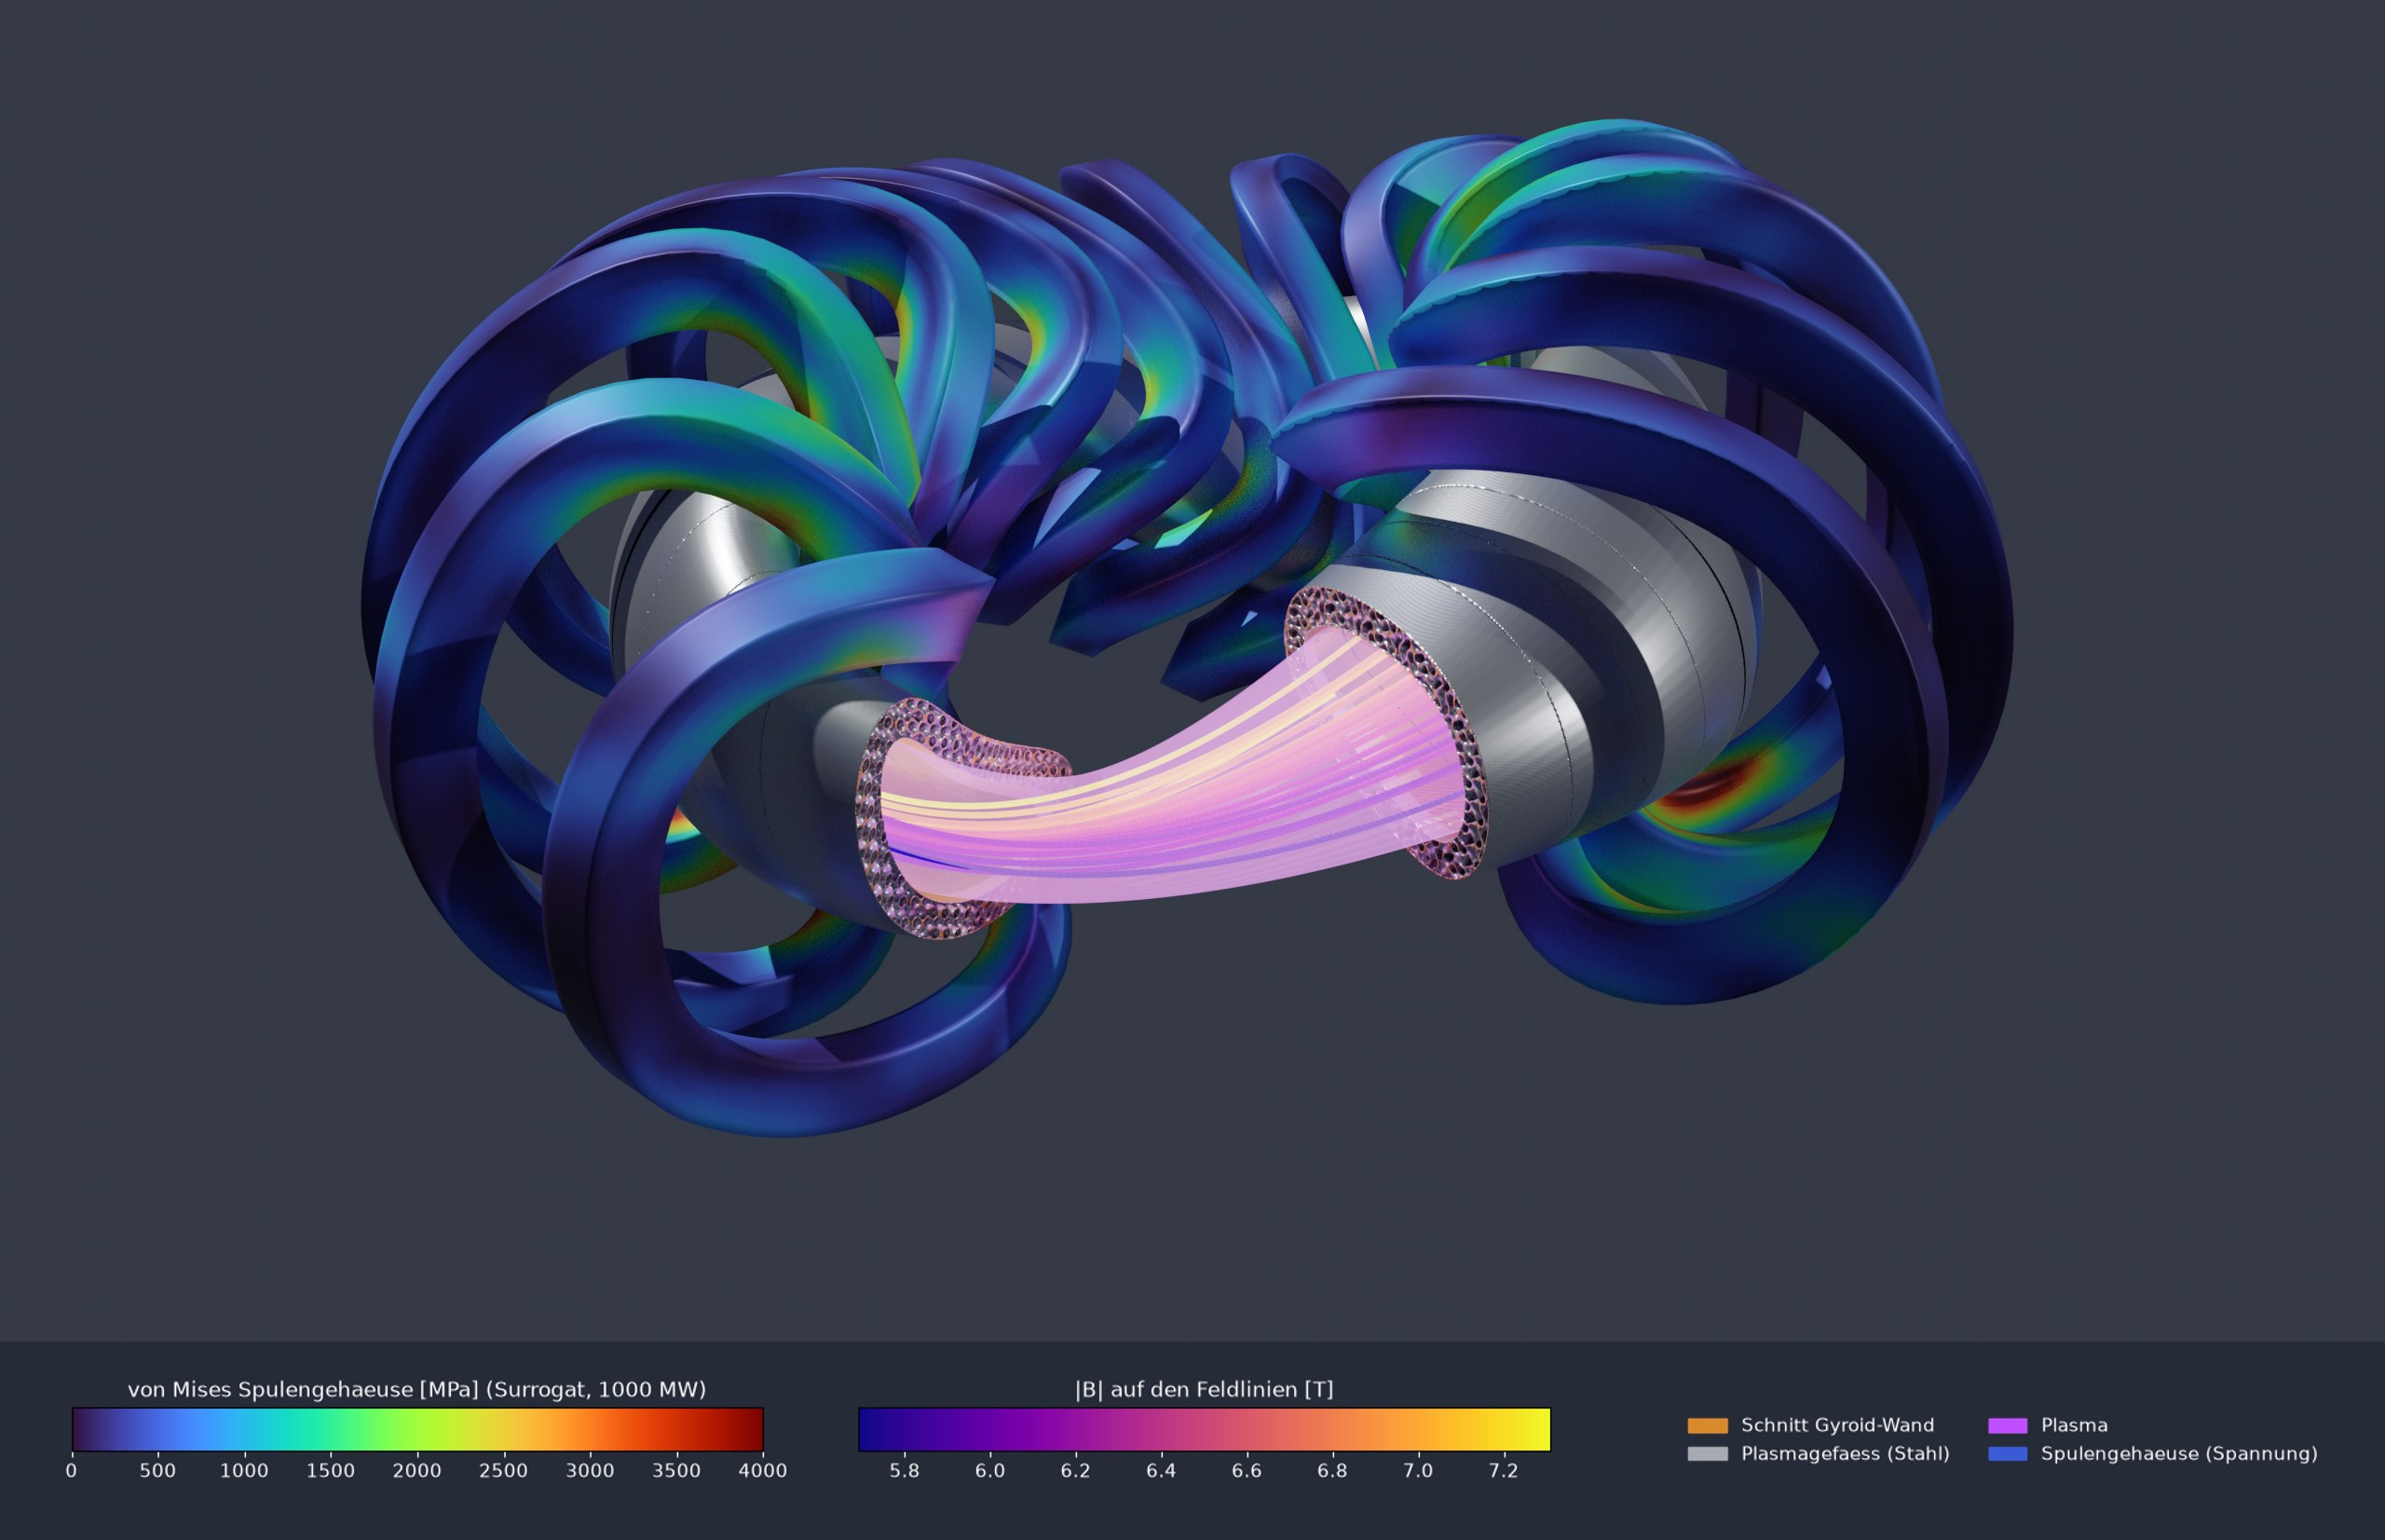
\includegraphics[width=\linewidth]{bilder/gyroid_gefaess_1GW_gesamt.jpg}
\caption{1-GW-Anlage frei im Raum: Spulengehäuse farbig nach Vergleichsspannung (Surrogat, \SI{1000}{MW}),
Plasmagefäß mit herausgeschnittenem Sektor; die Schnittflächen zeigen den Gyroid-Kern aus PicoGK. Feldlinien
(Biot-Savart) im Plasma, Farbe $|B|$. Drei Spulen über dem Ausschnitt und alle Verbinder ausgeblendet.}
\label{fig:gyroidgefaess}\end{figure}

%======================================================================
\section{Arbeitsweise: ein lokaler Agent als Aufsicht}
Der Rechenlauf dauerte mehrere Stunden. Damit dabei keine Rechenzeit eines großen Cloud-Modells verbraucht wird,
wurden die Rollen getrennt:
\begin{itemize}
\item \textbf{Claude Code} \cite{claudecode} baute Modell, Programm und Lauf und entschied über Änderungen.
\item Ein \textbf{Python-Lauf} rechnete ohne KI: Proben nacheinander, Ergebnisse sofort gesichert, Wiederaufnahme
  nach Absturz, Pause und Verlängerung über eine Steuerdatei, Speicher- und Plattenwächter.
\item \textbf{PI}, ein lokaler Coding-Agent \cite{pi} mit einem lokal betriebenen Qwen-Sprachmodell
  (27~Mrd.\ Parameter, über Ollama \cite{ollama}), sah alle 20 Minuten Fortschritt, Fehlerprotokoll und Laufzeiten
  an. Er durfte nur die Steuerdatei ändern (Pause, Stopp, Zeitgrenze, Löser, Probe überspringen) und musste
  jede Entscheidung im Format \emph{Zustand -- Beobachtung -- Eingriff} begründen. Am Ende schrieb er eine
  Zusammenfassung.
\end{itemize}
\kasten{Was PI tatsächlich tat.}{In allen Kontrollen meldete PI \glqq Zustand ok, Eingriff keiner\grqq{} und
begründete das richtig: Die beiden Fehlproben waren Einzelfälle ohne Serie, Laufzeiten weit unter der
Zeitgrenze. Seine Schlusszusammenfassung benannte von sich aus die schwächsten Kennzahlen (die Maxima). Eine
Antwort dauerte rund eine halbe Minute. Für den ersten Aufruf musste der Auftrag in eine Datei ausgelagert werden:
Ein langer Auftragstext mit Schrägstrichen wurde als Dateipfad gedeutet und brach ab.}

Weitere Erfahrungen aus dem Lauf: Eine geplante Pause des Menschen wurde per Zeitplan umgesetzt -- Lauf
angehalten, das Sprachmodell entladen, danach automatisch weiter. Einmal wurde der Arbeitsspeicher knapp,
weil neben einer großen W7-X-Probe noch eine Gitterzellen-Rechnung lief; seitdem prüft jedes Teilprogramm vor dem
Start den freien Speicher, und Teilrechnungen werden beim Abbruch mitbeendet. Ein Wiederanlaufskript stellt
nach einem Absturz den Sollzustand wieder her (Lauf fortsetzen, verwaiste Rechnungen beenden, Training
nachholen).

%======================================================================
\section{Fazit}
\begin{itemize}
\item Ein strukturiertes Hex-Netz fester Topologie ist der Schlüssel: Es macht ganze Felder lernbar und kommt
  ohne Vernetzer aus. Der Preis ist Handarbeit bei Verbindern und eine sorgfältige Prüfung der Elemente.
\item Rund 80 Rechnungen je Anlage genügen für robuste Kennzahlen (99-\%-Wert, Masse, Verformung: wenige Prozent
  Fehler). Lokale Spitzen bleiben Sache der FEM.
\item Die Empfindlichkeiten sind für den Konstrukteur direkt lesbar: Bei der W7-X-ähnlichen Anlage zuerst die
  Seitenwand verstärken; bei 1~GW hilft keine Wandstärke im untersuchten Bereich -- das Tragkonzept muss sich ändern.
\item Ein kleiner lokaler Agent als Aufsicht über einen deterministischen Lauf funktioniert, wenn seine Rechte
  eng begrenzt sind und er begründen muss. Die eigentliche Robustheit liefert der Lauf selbst.
\end{itemize}
\subsection*{Offene Punkte}
Widerspruch zum Tetraedermodell (Lagerung, B-027); realistischere Lagerung; voller Steifigkeitstensor der
Gitterzellen und Gitterfüllung im 1-GW-Modell; Plasmagefäß mit Gyroid-Kühlkern (Geometrie begonnen).

\subsection*{Software und Daten}
ElmerFEM \cite{elmer} mit MUMPS \cite{mumps}, scikit-learn \cite{sklearn}, PicoGK \cite{picogk}, PyVista
\cite{pyvista}, simsopt \cite{simsopt}. Programmcode (u.\,a.\ \texttt{stellarator/hexmodell.py},
\texttt{surrogat.py}, \texttt{surrogat\_waechter.py}, \texttt{gitterzelle.py}) und Befundprotokoll:
\url{https://github.com/ThomasSchmiegelt/stellarator-design} (MIT-Lizenz).

\begin{thebibliography}{99}\small
\bibitem{simsopt} M. Landreman, B. Medasani, F. Wechsung, A. Giuliani, R. Jorge, C. Zhu: SIMSOPT: A flexible
  framework for stellarator optimization. \emph{J.\ Open Source Softw.} 6(65) (2021) 3525.
  doi:10.21105/joss.03525.
\bibitem{elmer} ElmerFEM, Version 9.0. CSC -- IT Center for Science, Finnland. \url{https://www.elmerfem.org}
\bibitem{mumps} P.\,R. Amestoy, I.\,S. Duff, J.-Y. L'Excellent, J. Koster: A fully asynchronous multifrontal
  solver using distributed dynamic scheduling. \emph{SIAM J.\ Matrix Anal.\ Appl.} 23(1) (2001) 15--41.
\bibitem{mckay1979} M.\,D. McKay, R.\,J. Beckman, W.\,J. Conover: A comparison of three methods for selecting
  values of input variables in the analysis of output from a computer code. \emph{Technometrics} 21(2) (1979)
  239--245.
\bibitem{rasmussen2006} C.\,E. Rasmussen, C.\,K.\,I. Williams: \emph{Gaussian Processes for Machine Learning}.
  MIT Press (2006).
\bibitem{sklearn} F. Pedregosa et al.: Scikit-learn: Machine learning in Python. \emph{J.\ Mach.\ Learn.\ Res.}
  12 (2011) 2825--2830.
\bibitem{gibson1997} L.\,J. Gibson, M.\,F. Ashby: \emph{Cellular Solids: Structure and Properties}, 2.\ Aufl.
  Cambridge University Press (1997).
\bibitem{blender} Blender, Version 4.0. Blender Foundation. \url{https://www.blender.org}
\bibitem{picogk} LEAP 71: PicoGK. \url{https://github.com/LEAP71/PicoGK} (Apache-2.0-Lizenz).
\bibitem{pyvista} C.\,B. Sullivan, A. Kaszynski: PyVista: 3D plotting and mesh analysis through a streamlined
  interface for the Visualization Toolkit (VTK). \emph{J.\ Open Source Softw.} 4(37) (2019) 1450.
\bibitem{pi} M. Zechner: pi coding agent. \url{https://github.com/earendil-works/pi} (MIT-Lizenz).
\bibitem{ollama} Ollama. \url{https://ollama.com}
\bibitem{claudecode} Anthropic: Claude Code. \url{https://www.anthropic.com/claude-code}
\end{thebibliography}
\end{document}
